\section{Using a virtual circuit per file-transfer}

\subsection{Integrating FDT into PhEDEx}
The FDT tool integrates InterDomain Controller Protocol (IDCP)
On-Demand Secure Circuits and Advance Reservation System (OSCARS\cite{OSCARS}) calls so
integrating it in PhEDEx naturally gives us Bandwidth on Demand
capabilities. In addition to this, FDT performs extremely well
as a transfer tool in itself, as we will show in this paper.

As shown in Figure \ref{fig:PhEDEx-FDT-arch}, the current architecture consists
of four main components:
\begin{description}
	\item[FDT tool] - written in Java it's based on an asynchronous, flexible 
multithreaded system, using the capabilities of the Java NIO 
libraries. It's capable of reading and writing at disk speed over wide area 
networks and runs on all major platforms. 
	\item[PhEDEx backend] - written in Perl, this backend
receives transfer jobs from the FileDownload site agent which will, in turn, 
invoke the fdtcp wrapper. 
	\item[Fdtcp wrapper] - written in Python this is the
interface between PhEDEx and FDT. It prepares the file list as required by FDT, 
invokes the fdtd service and harvests reports to be propagated back to PhEDEx.
	\item[Fdtcp daemon] - written in Python as well, it's
a permanently running daemon, responsible for authentication and completion of requests
from fdtcp. These requests are transmitted via PYthon Remote Objects (PYRO)
calls and will either launch FDT in client mode on source sites or in server
mode on destination sites.
\end{description}

\begin{figure}[h]
  \centering
  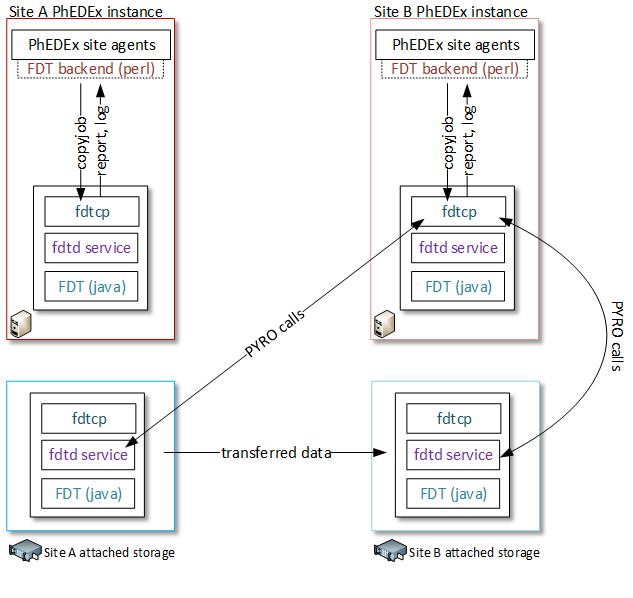
\includegraphics[width=0.95\textwidth]{Figures/PhEDEx-and-FDT-diagram.png}
  \caption{Diagram of various components needed to integrate FDT into PhEDEx}
  \label{fig:PhEDEx-FDT-arch}
\end{figure} 

Figure \ref{fig:PhEDEx-FDT-arch} also describes a normal scenario in which Site B
needs to transfer data from Site A. In this example, the PhEDEx instance and the
storage node are separate physical servers. 

The FileDownload agent on the PhEDEx server on Site A gets a list of files to
transfer from the PhEDEx database. It breaks the list (up to 10 PB of data) into
manageable chunks (up to a few TB of data) and
hands the chunks to the FDT backend. The FDT backend on that machine will then issue an fdtcp
command for each group of files to copy those files from the storage node of
Site A to the storage node of Site B.

Fdtcp will, in turn, invoke the \emph{fdtd} daemons on the two storage nodes. Each fdtd
daemon will first verify that the command comes from an approved server, after
which it will launch the appropriate FDT tool. The fdtd daemon on Site B
will start the FDT tool in server mode and the daemon on site B starts FDT in 
client mode.

Once this is done, the transfers are handled by FDT. After the transfer finishes
the reports are then propagated up the chain, eventually reaching PhEDEx.

\subsection{Testbed configuration and transfer results with FDT}

\subsubsection{Testbed configuration}

The tests were run on our testbed (Figure \ref{fig:ANSE-setup}), using the Geneva
(T2\_ANSE\_Geneva) and Amsterdam (T2\_ANSE\_Amsterdam) sites. All LSI controllers
were used.

Each transfer job was 2.25TB (150x15TB files).

\subsubsection{Transfer results with FDT}

As seen in Figure \ref{fig:FDT-Transfers} and Figure \ref{fig:FDT-Transfers-PhEDEx}
FDT is able to achieve sustained rates of over 1500MB/sec. As PhEDEx shows,
the average sits at a marginally slower 1360MB/sec. Figure \ref{fig:FDT-Transfers}, shows periodic drops in transfer rates.
This is due to the fact that between each transfer job (which is composed of a limited
number of files) there is a delay between the ending of one job and the launch of
a new one. This is what accounts for the difference in average reported rates by PhEDEx
and the average rate for each transfer job. This is an artifact of our configuration, which only allowed one
transfer job to run at a time. In a production environment PhEDEx would run overlapping jobs, so this structure would not be apparent. Nonetheless, we chose to keep the simpler configuration for these first tests, so that results would be easy to interpret.

These high transfer rates are not only due to the storage system alone. FDT
automatically starts the correct number of readers and writers if the files at 
the source and destinations sites are spread on different physical disks/controllers.

\begin{figure}[h]
  \centering
  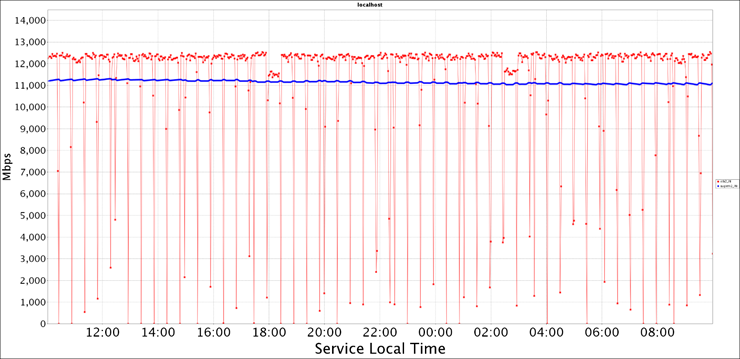
\includegraphics[width=0.95\textwidth]{Figures/FDT-transfers.png}
  \caption{PhEDEx transfers over 24hrs using FDT as reported by MonALISA. 
  The red line represents the network interface throughput in Mbit/sec, with data points
  each minute. The blue line represents a moving average over one hour of that throughput.}
  \label{fig:FDT-Transfers}
\end{figure} 

\begin{figure}[h]
  \centering
  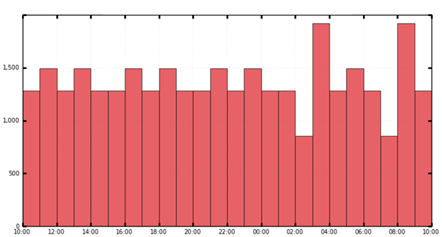
\includegraphics[width=0.95\textwidth]{Figures/FDT-transfers-PhEDEx.png}
  \caption{PhEDEx transfers over 24hrs using FDT as reported by PhEDEx. Transfer rates are
  given in MB/sec, with one hour bins. This, coupled with the fact that rates are only 
  reported at the end of job transfers, make this plot look bumpy.}
  \label{fig:FDT-Transfers-PhEDEx}
\end{figure} 


\subsubsection{Limitations of the current testbed}

At the moment this system does have some drawbacks:

\begin{itemize}
  \item As noted, The PhEDEx agent configuration has been simplified, compared to the production environment, for ease of comprehension.
	\item FDT requires a POSIX compatible interface to function. At the moment
not all PhEDEx sites provide such an interface to their storage elements, so FDT is not actually deployed by CMS at this time.
	\item In order to get the best performance out of the systems, files that
are to be transfered need to be spread among different disks on both source
and destination storage servers. This adds more complexity to the sites'
configuration and operation.
\end{itemize}

Despite these limitations - or rather because of them - this testbed is a valuable resource for understanding the behaviour of PhEDEx when we attempt to push its transfer performance to the limit.